\chapter{Implementation, integration and test plan}

\section{Development process and approach}

The system will be implemented, integrated, and tested following a bottom-up approach, starting from the model layer and progressively adding and testing the other components of the server architecture.
This approach allows for the early validation of low-level functionalities, ensuring a solid foundation for higher-level components.

Both server-side and client-side components will be developed and tested simultaneously, but the focus will be on server-side components initially, due to their backbone role of the system.
Incremental integration testing will be applied, aiming to identify and resolve bugs as soon as they emerge during the development process, minimizing the impact on subsequent stages.

To facilitate testing at different levels of the architecture, drivers will be employed to simulate higher-level components that are not yet implemented, while stubs will be used to mock the behavior of lower-level dependencies, such as external services or the database.
This strategy ensures that individual components can be tested in isolation, while also validating their integration as part of the broader system.

This testing approach ensures that dependencies between components are carefully managed, leading to a robust and well-tested system at every level.

\section{Implementation and integeration plan}

This section describes the implementation and integration plan of each part of the system.

\subsection{Application server}

Firstly, the model and the query service will be implemented and unit tested with a driver, which will substitute components not yet implemented.

\begin{figure}[H]
    \centering
    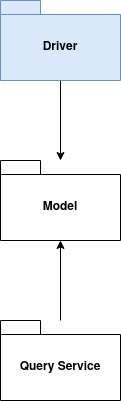
\includegraphics[width=0.1\linewidth]{../../assets/implementation-plan-diagrams/implementation-plan-1.png}
\end{figure}

As the second step, the authentication service, profile manager, recommendation service, enrollment manager and internship manager will be implemented and tested with a driver, which will substitute the request dispatcher.

There will also be 3 stubs, which will substitute, respectively, the email service for the authentication service, the suggestion service for the profile manager, and the complaint manager and feedback manager for the internship manager.

\begin{figure}[H]
    \centering
    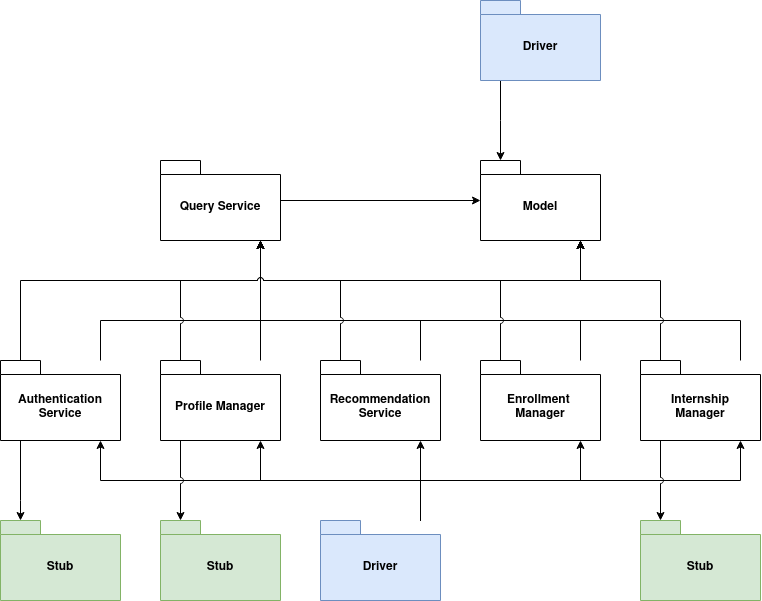
\includegraphics[width=0.7\linewidth]{../../assets/implementation-plan-diagrams/implementation-plan-2.png}
\end{figure}

Then, the request dispatcher will be implemented and tested with a driver substituting the web server.

\begin{figure}[H]
    \centering
    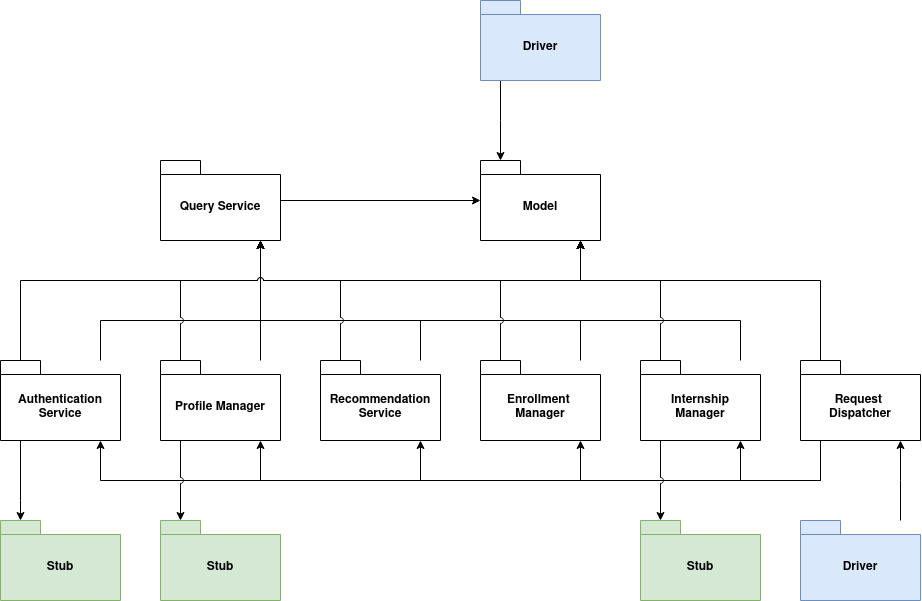
\includegraphics[width=0.8\linewidth]{../../assets/implementation-plan-diagrams/implementation-plan-3.png}
\end{figure}

the last components of the server that will be implemented will be the email service, the suggestion service, the complaint manager and the feedback manager.
A stub will be used to simulate the behavior of the email server.

\begin{figure}[H]
    \centering
    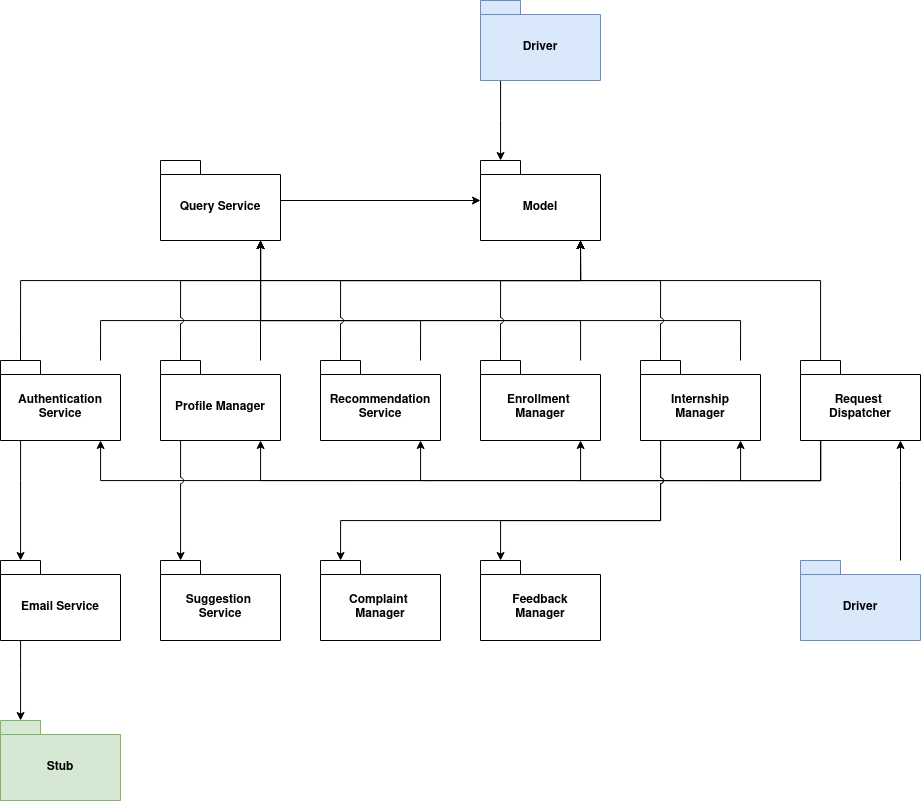
\includegraphics[width=0.8\linewidth]{../../assets/implementation-plan-diagrams/implementation-plan-4.png}
\end{figure}

\subsection{Web server}

Each component of the view is rigorously unit tested using a stub for the REST APIs, enabling parallel development of the frontend and backend.

\begin{figure}[H]
    \centering
    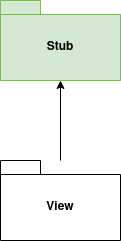
\includegraphics[width=0.1\linewidth]{../../assets/implementation-plan-diagrams/implementation-plan-5.png}
\end{figure}

\subsection{Final test}

Once the implementations of the backend and of the frontend are finished, final tests can take place.

\begin{figure}[H]
    \centering
    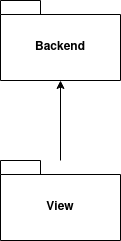
\includegraphics[width=0.1\linewidth]{../../assets/implementation-plan-diagrams/implementation-plan-6.png}
\end{figure}

